\chapter{Vectors and Vector Calculus}
\label{ch:vectors}
\begin{chapterintro}
\textbf{You will learn to:} add and subtract vectors; resolve them into
components; compute scalar and vector products; differentiate vector functions;
and use the gradient, divergence, and curl. These operations are the grammar of
mechanics: position, velocity, force, torque, and work are all built from them.
\end{chapterintro}

\section{Scalars and vectors}

A \textbf{scalar} is fully described by a number and a unit: mass, time,
temperature, energy. A \textbf{vector} also has a direction and a sense: position,
velocity, acceleration, force, momentum.

A vector $\vec{A}$ is written in the Cartesian basis $(\ihat,\jhat,\khat)$ as
\[
\vec{A}=A_x\ihat+A_y\jhat+A_z\khat.
\]
Its magnitude is
\[
\norm{\vec{A}}=\sqrt{A_x^2+A_y^2+A_z^2},
\]
and its unit vector is $\vec{u}_A=\vec{A}/\norm{\vec{A}}$.

\begin{figure}[htbp]
\centering
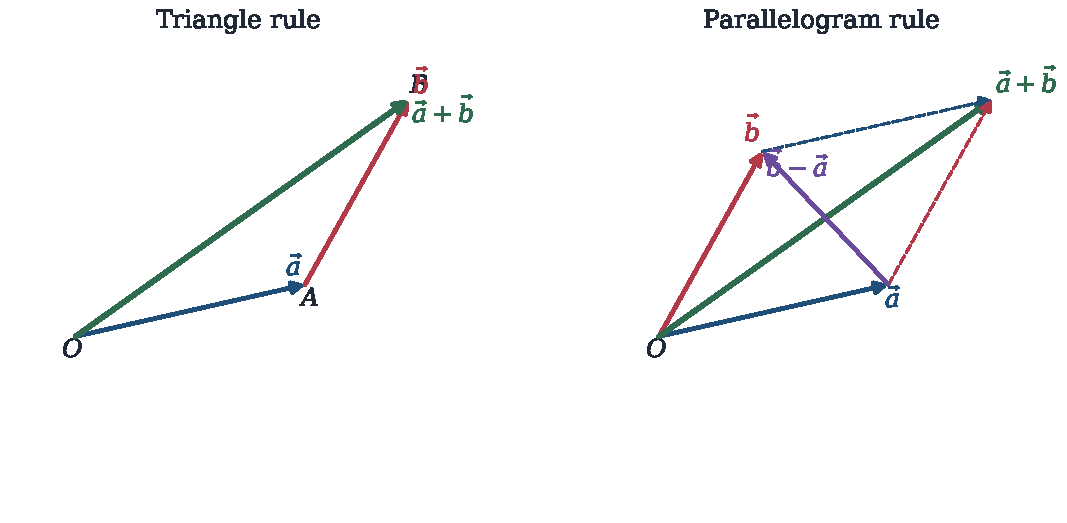
\includegraphics[width=0.95\textwidth]{figures/01_vector_addition.pdf}
\caption{Two equivalent constructions for the sum of two vectors. The difference
$\vec b-\vec a$ is the vector that must be added to $\vec a$ to obtain $\vec b$.}
\label{fig:vector-addition}
\end{figure}

\section{Vector algebra}

\subsection{Addition and subtraction}
Component by component:
\[
\vec{A}\pm\vec{B}=(A_x\pm B_x)\ihat+(A_y\pm B_y)\jhat+(A_z\pm B_z)\khat.
\]
Graphically, use the triangle or parallelogram rule
(\cref{fig:vector-addition}). Addition is commutative and associative.

\subsection{Scalar (dot) product}
\[
\vec{A}\cdot\vec{B}
=\norm{\vec{A}}\norm{\vec{B}}\cos\theta
=A_xB_x+A_yB_y+A_zB_z.
\]
The result is a scalar. In particular,
\[
\vec{A}\cdot\vec{B}=0\iff\vec{A}\perp\vec{B},
\qquad
\vec{A}\cdot\vec{A}=\norm{\vec{A}}^2.
\]
The projection of $\vec B$ onto the direction of $\vec A$ is
$B\cos\theta=(\vec A\cdot\vec B)/\norm{\vec A}$.

\begin{figure}[htbp]
\centering
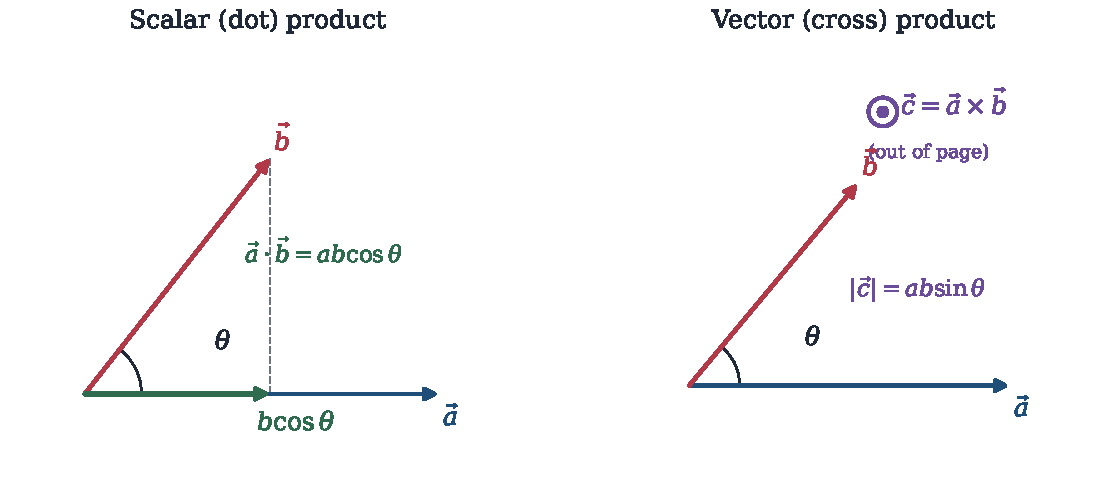
\includegraphics[width=0.95\textwidth]{figures/03_dot_cross.pdf}
\caption{The scalar product measures projection; the vector product measures the
area of the parallelogram and points along the right-hand normal.}
\label{fig:dot-cross}
\end{figure}

\subsection{Vector (cross) product}
\[
\vec{A}\times\vec{B}
=\begin{vmatrix}
\ihat & \jhat & \khat\\
A_x & A_y & A_z\\
B_x & B_y & B_z
\end{vmatrix},
\qquad
\norm{\vec{A}\times\vec{B}}
=\norm{\vec{A}}\norm{\vec{B}}\sin\theta.
\]
The result is a vector perpendicular to both $\vec A$ and $\vec B$, oriented by the
right-hand rule (\cref{fig:dot-cross}). The product is anti-commutative:
$\vec A\times\vec B=-(\vec B\times\vec A)$. Moreover,
\[
\vec{A}\times\vec{B}=\vzero\iff\vec{A}\parallel\vec{B}.
\]

\subsection{Triple products}
The scalar triple product gives the signed volume of the parallelepiped built on
the three vectors:
\[
\vec{A}\cdot(\vec{B}\times\vec{C})
=\begin{vmatrix}
A_x&A_y&A_z\\
B_x&B_y&B_z\\
C_x&C_y&C_z
\end{vmatrix}.
\]
The vector triple product satisfies
\[
\vec{A}\times(\vec{B}\times\vec{C})
=(\vec{A}\cdot\vec{C})\vec{B}-(\vec{A}\cdot\vec{B})\vec{C}.
\]

\section{Vector functions and their derivatives}

If a vector depends on time, $\vec{A}(t)=A_x(t)\ihat+A_y(t)\jhat+A_z(t)\khat$,
then
\[
\frac{\dd\vec{A}}{\dd t}
=\dot A_x\ihat+\dot A_y\jhat+\dot A_z\khat.
\]
The usual rules hold:
\[
\frac{\dd}{\dd t}(\vec A+\vec B)=\dot{\vec A}+\dot{\vec B},\qquad
\frac{\dd}{\dd t}(\vec A\cdot\vec B)
=\dot{\vec A}\cdot\vec B+\vec A\cdot\dot{\vec B},
\]
\[
\frac{\dd}{\dd t}(\vec A\times\vec B)
=\dot{\vec A}\times\vec B+\vec A\times\dot{\vec B}.
\]

\begin{keyidea}[Why derivatives matter]
Velocity is the time derivative of the position vector and acceleration is the
time derivative of velocity. Master the differentiation of vectors and kinematics
becomes bookkeeping.
\end{keyidea}

\section{Differential operators}

For a scalar field $f(x,y,z)$ and a vector field
$\vec{V}=V_x\ihat+V_y\jhat+V_z\khat$:

\begin{align*}
\grad f &= \frac{\partial f}{\partial x}\ihat
+\frac{\partial f}{\partial y}\jhat
+\frac{\partial f}{\partial z}\khat,\\[2pt]
\divg\vec V &= \frac{\partial V_x}{\partial x}
+\frac{\partial V_y}{\partial y}
+\frac{\partial V_z}{\partial z},\\[2pt]
\rot\vec V &=
\begin{vmatrix}
\ihat & \jhat & \khat\\[2pt]
\dfrac{\partial}{\partial x} & \dfrac{\partial}{\partial y} & \dfrac{\partial}{\partial z}\\[4pt]
V_x & V_y & V_z
\end{vmatrix},\\[2pt]
\Delta f &= \divg(\grad f)
=\frac{\partial^2f}{\partial x^2}
+\frac{\partial^2f}{\partial y^2}
+\frac{\partial^2f}{\partial z^2}.
\end{align*}

Two identities are used repeatedly:
\[
\rot(\grad f)=\vzero,\qquad \divg(\rot\vec V)=0.
\]
The first says that every gradient field is irrotational; it is the mathematical
basis of conservative forces in \cref{ch:energy}.

\begin{figure}[htbp]
\centering
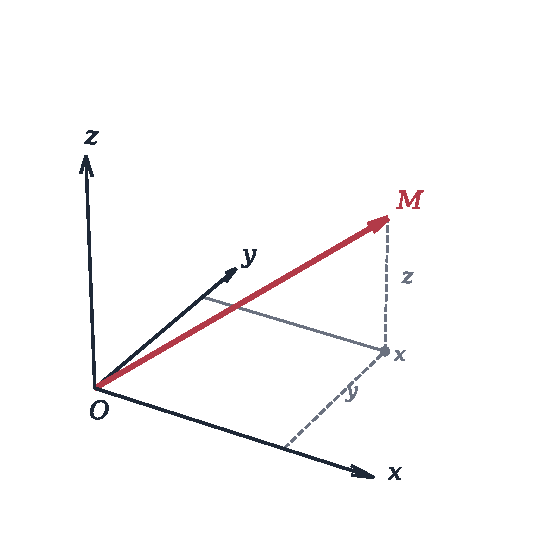
\includegraphics[width=0.72\textwidth]{figures/02_cartesian_3d.pdf}
\caption{The Cartesian components of the position vector $\vec{OM}$.}
\label{fig:cartesian}
\end{figure}

% ===========================================================================
\section{Worked examples}

\begin{worked}[Full vector algebra]
Let $\vec A=2\ihat-3\jhat+\khat$ and $\vec B=-\ihat+4\jhat-2\khat$. Compute
$\vec A+\vec B$, $\norm{\vec A}$, $\vec A\cdot\vec B$, the angle between them, and
$\vec A\times\vec B$.
\end{worked}

\begin{solution}{2.1}
\[
\vec A+\vec B=(2-1)\ihat+(-3+4)\jhat+(1-2)\khat
=\ihat+\jhat-\khat.
\]
\[
\norm{\vec A}=\sqrt{2^2+(-3)^2+1^2}=\sqrt{14}=3.74.
\]
\[
\vec A\cdot\vec B=(2)(-1)+(-3)(4)+(1)(-2)
=-2-12-2=-16.
\]
Since $\vec A\cdot\vec B=\norm{\vec A}\norm{\vec B}\cos\theta$ and
$\norm{\vec B}=\sqrt{1+16+4}=\sqrt{21}=4.58$,
\[
\cos\theta=\frac{-16}{\sqrt{14}\sqrt{21}}
=\frac{-16}{17.15}=-0.933,
\qquad
\theta=159^\circ.
\]
Finally,
\[
\vec A\times\vec B=
\begin{vmatrix}
\ihat&\jhat&\khat\\
2&-3&1\\
-1&4&-2
\end{vmatrix}
=(6-4)\ihat-(-4+1)\jhat+(8-3)\khat
=2\ihat+3\jhat+5\khat.
\]
Check: $(2,3,5)\cdot(2,-3,1)=4-9+5=0$ and
$(2,3,5)\cdot(-1,4,-2)=-2+12-10=0$.
\end{solution}

\begin{worked}[Gradient and conservative field]
For $f(x,y,z)=x^2y+yz^3$, compute $\grad f$ at $P(1,2,-1)$. Then find the force
field $\vec F=-\grad f$ and verify that $\rot\vec F=\vzero$.
\end{worked}

\begin{solution}{2.2}
\[
\frac{\partial f}{\partial x}=2xy,\qquad
\frac{\partial f}{\partial y}=x^2+z^3,\qquad
\frac{\partial f}{\partial z}=3yz^2.
\]
At $(1,2,-1)$:
\[
\grad f=(4)\ihat+(1-1)\jhat+(3\cdot2\cdot1)\khat
=4\ihat+6\khat.
\]
Thus $\vec F=-4\ihat-6\khat$ at $P$. Since $\vec F=-\grad f$ is a gradient
field, $\rot\vec F=-\rot(\grad f)=\vzero$ identically. Directly,
\[
\vec F=(-2xy,-x^2-z^3,-3yz^2),
\]
and each component of the curl cancels.
\end{solution}

% ===========================================================================
\section{Exercises and Step-by-Step Solutions}

\begin{exercise}{\warm\ Components and magnitude}
Let $\vec A=3\ihat+4\jhat$ and $\vec B=-2\ihat+5\jhat$. Find
$\vec A+\vec B$, $\vec A-\vec B$, $\norm{\vec A}$, $\norm{\vec B}$, and the unit
vectors $\vec u_A$ and $\vec u_B$.
\end{exercise}

\begin{tabletworkspace}[6.5cm]
\end{tabletworkspace}

\begin{solution}{2.1}
\[
\vec A+\vec B=(3-2)\ihat+(4+5)\jhat=\ihat+9\jhat,
\]
\[
\vec A-\vec B=(3+2)\ihat+(4-5)\jhat=5\ihat-\jhat.
\]
\[
\norm{\vec A}=\sqrt{9+16}=5,\qquad \norm{\vec B}=\sqrt{4+25}=\sqrt{29}=5.39.
\]
\[
\vec u_A=\frac{3}{5}\ihat+\frac{4}{5}\jhat,\qquad
\vec u_B=\frac{-2}{\sqrt{29}}\ihat+\frac{5}{\sqrt{29}}\jhat.
\]
\end{solution}

\begin{exercise}{\warm\ Dot product and angle}
For $\vec A=(1,2,3)$ and $\vec B=(4,-5,6)$, compute $\vec A\cdot\vec B$ and the
angle between the two vectors.
\end{exercise}

\begin{tabletworkspace}[6.5cm]
\end{tabletworkspace}

\begin{solution}{2.2}
\[
\vec A\cdot\vec B=4-10+18=12.
\]
\[
\norm{\vec A}=\sqrt{14}=3.742,\qquad \norm{\vec B}=\sqrt{77}=8.775.
\]
\[
\cos\theta=\frac{12}{(3.742)(8.775)}=0.3655,
\qquad \theta=68.6^\circ.
\]
\end{solution}

\begin{exercise}{\warm\ Cross product and area}
For $\vec A=(3,1,0)$ and $\vec B=(1,2,-1)$, compute $\vec A\times\vec B$ and the
area of the parallelogram spanned by the two vectors.
\end{exercise}

\begin{tabletworkspace}[6.5cm]
\end{tabletworkspace}

\begin{solution}{2.3}
\[
\vec A\times\vec B=
\begin{vmatrix}
\ihat&\jhat&\khat\\
3&1&0\\
1&2&-1
\end{vmatrix}
=(-1-0)\ihat-( -3-0)\jhat+(6-1)\khat
=-\ihat+3\jhat+5\khat.
\]
The area is
\[
\norm{\vec A\times\vec B}=\sqrt{1+9+25}=\sqrt{35}=5.92.
\]
\end{solution}

\begin{exercise}{\core\ Perpendicular and parallel conditions}
(a) Find $\lambda$ such that $\vec A=(2,\lambda,1)$ is perpendicular to
$\vec B=(3,-1,2)$. (b) Find $\mu$ such that $\vec C=(\mu,-1,2)$ is parallel to
$\vec B$.
\end{exercise}

\begin{tabletworkspace}[6.5cm]
\end{tabletworkspace}

\begin{solution}{2.4}
(a) Perpendicularity requires $\vec A\cdot\vec B=0$:
\[
(2)(3)+(\lambda)(-1)+(1)(2)=0
\implies 8-\lambda=0
\implies \lambda=8.
\]
(b) Parallelism requires $\vec C$ to be a multiple of $\vec B$. The second
component already matches, so the multiplier is $1$; hence $\mu=3$.
\end{solution}

\begin{exercise}{\core\ Scalar triple product}
For $\vec A=(1,0,2)$, $\vec B=(2,1,0)$, and $\vec C=(0,3,1)$, compute
$\vec A\cdot(\vec B\times\vec C)$ and the volume of the parallelepiped they
define.
\end{exercise}

\begin{tabletworkspace}[6.5cm]
\end{tabletworkspace}

\begin{solution}{2.5}
\[
\vec B\times\vec C=
\begin{vmatrix}
\ihat&\jhat&\khat\\
2&1&0\\
0&3&1
\end{vmatrix}
=\ihat-2\jhat+6\khat.
\]
\[
\vec A\cdot(\vec B\times\vec C)
=(1)(1)+(0)(-2)+(2)(6)=13.
\]
The volume is $\abs{13}=13$ cubic units.
\end{solution}

\begin{exercise}{\core\ Vector triple product}
Verify the identity
$\vec A\times(\vec B\times\vec C)=(\vec A\cdot\vec C)\vec B-(\vec A\cdot\vec B)\vec C$
for $\vec A=(1,2,0)$, $\vec B=(0,1,3)$, and $\vec C=(2,0,1)$.
\end{exercise}

\begin{tabletworkspace}[6.5cm]
\end{tabletworkspace}

\begin{solution}{2.6}
First,
\[
\vec B\times\vec C=
\begin{vmatrix}
\ihat&\jhat&\khat\\
0&1&3\\
2&0&1
\end{vmatrix}
=\ihat+6\jhat-2\khat.
\]
Then
\[
\vec A\times(\vec B\times\vec C)=
\begin{vmatrix}
\ihat&\jhat&\khat\\
1&2&0\\
1&6&-2
\end{vmatrix}
=(-4)\ihat-( -2)\jhat+(6-2)\khat
=-4\ihat+2\jhat+4\khat.
\]
On the other hand, $\vec A\cdot\vec C=2$ and $\vec A\cdot\vec B=2$, so
\[
2\vec B-2\vec C=(0,2,6)-(4,0,2)=(-4,2,4).
\]
The two results agree.
\end{solution}

\begin{exercise}{\core\ Differentiating a vector}
A particle has position $\vec r(t)=(3t^2,2t,t^3)$ (SI units). Find its velocity
and acceleration at $t=1.00\ \mathrm{s}$, and the magnitudes of both.
\end{exercise}

\begin{tabletworkspace}[6.5cm]
\end{tabletworkspace}

\begin{solution}{2.7}
\[
\vec v(t)=\dot{\vec r}=(6t,2,3t^2),\qquad
\vec a(t)=\ddot{\vec r}=(6,0,6t).
\]
At $t=1$:
\[
\vec v=(6,2,3)\ \mathrm{m\,s^{-1}},\qquad
\norm{\vec v}=\sqrt{36+4+9}=7.00\ \mathrm{m\,s^{-1}},
\]
\[
\vec a=(6,0,6)\ \mathrm{m\,s^{-2}},\qquad
\norm{\vec a}=\sqrt{36+36}=8.49\ \mathrm{m\,s^{-2}}.
\]
\end{solution}

\begin{exercise}{\core\ Gradient}
For $f(x,y,z)=x^2+y^2+z^2$, compute $\grad f$ at $P(1,2,2)$, its magnitude, and
the unit vector in the direction of steepest increase.
\end{exercise}

\begin{tabletworkspace}[6.5cm]
\end{tabletworkspace}

\begin{solution}{2.8}
\[
\grad f=(2x,2y,2z).
\]
At $P(1,2,2)$:
\[
\grad f=(2,4,4),\qquad \norm{\grad f}=\sqrt{4+16+16}=6.00.
\]
The direction of steepest increase is
\[
\vec u=\frac{1}{6}(2,4,4)=\left(\frac13,\frac23,\frac23\right).
\]
\end{solution}

\begin{exercise}{\mastery\ Divergence and curl}
For $\vec V=(x^2y,\,yz^2,\,xz)$, compute $\divg\vec V$ and $\rot\vec V$, and
verify explicitly that $\divg(\rot\vec V)=0$.
\end{exercise}

\begin{tabletworkspace}[6.5cm]
\end{tabletworkspace}

\begin{solution}{2.9}
\[
\divg\vec V=\frac{\partial}{\partial x}(x^2y)
+\frac{\partial}{\partial y}(yz^2)
+\frac{\partial}{\partial z}(xz)
=2xy+z^2+x.
\]
For the curl,
\[
\rot\vec V=
\left(
\frac{\partial V_z}{\partial y}-\frac{\partial V_y}{\partial z},
\frac{\partial V_x}{\partial z}-\frac{\partial V_z}{\partial x},
\frac{\partial V_y}{\partial x}-\frac{\partial V_x}{\partial y}
\right)
=(-2yz,\,-z,\,-x^2).
\]
Then
\[
\divg(\rot\vec V)
=\frac{\partial(-2yz)}{\partial x}
+\frac{\partial(-z)}{\partial y}
+\frac{\partial(-x^2)}{\partial z}
=0.
\]
\end{solution}

\begin{exercise}{\mastery\ Recovering a potential}
Show that
$\vec F=(y^2,\,2xy+z,\,y)$
is conservative, then find a scalar function $\varphi(x,y,z)$ such that
$\vec F=\grad\varphi$.
\end{exercise}

\begin{tabletworkspace}[6.5cm]
\end{tabletworkspace}

\begin{solution}{2.10}
Write $\vec F=(F_x,F_y,F_z)=(y^2,\,2xy+z,\,y)$. Compute
\[
\rot\vec F=
\left(
\frac{\partial F_z}{\partial y}-\frac{\partial F_y}{\partial z},
\frac{\partial F_x}{\partial z}-\frac{\partial F_z}{\partial x},
\frac{\partial F_y}{\partial x}-\frac{\partial F_x}{\partial y}
\right)
=(1-1,\,0-0,\,2y-2y)=\vzero.
\]
The field is irrotational, hence conservative. To find $\varphi$:
\[
\frac{\partial\varphi}{\partial x}=y^2
\implies \varphi=xy^2+g(y,z).
\]
Then
\[
\frac{\partial\varphi}{\partial y}=2xy+\frac{\partial g}{\partial y}=2xy+z
\implies \frac{\partial g}{\partial y}=z
\implies g=yz+h(z).
\]
Finally
\[
\frac{\partial\varphi}{\partial z}=y+h'(z)=y
\implies h'(z)=0.
\]
Thus
\[
\varphi(x,y,z)=xy^2+yz+C.
\]
\end{solution}

